%%%%%%%%%%%%%%%%%%%%%%%%%%%%%%%%%%%%%%%%%%%%%%%%%%%%%%%%%%%%%%%%%%%%%%%%%%%%%%%%
%2345678901234567890123456789012345678901234567890123456789012345678901234567890
%        1         2         3         4         5         6         7         8

\documentclass[letterpaper, 10 pt, conference]{ieeeconf}
  % use above line letter sized paper
%\documentclass[a4paper, 10pt, conference]{ieeeconf}
  % Use this line for a4 paper
\IEEEoverridecommandlockouts
  % Needed if you want to use the \thanks command
\overrideIEEEmargins
  % Needed to meet printer requirements.


% The following packages can be found on http:\\www.ctan.org
\usepackage{graphicx} % for pdf, bitmapped graphics files


\usepackage{epsfig} % for postscript graphics files
%\usepackage{mathptmx} % assumes new font selection scheme installed
%\usepackage{times} % assumes new font selection scheme installed
\usepackage{amsmath} % assumes amsmath package installed
\usepackage{amssymb}  % assumes amsmath package installed
\usepackage{pstricks}
\usepackage[utf8]{inputenc}
\usepackage{color}
\usepackage[font=footnotesize,caption=false]{subfig}
\usepackage[caption=false,font=footnotesize]{subfig}
\usepackage{hyperref}

\newcommand{\TODO}[1]{\textcolor{green}{TODO : #1}} %pour lister ce qu'il reste à faire
\newcommand{\CD}[2]{\textcolor{red}{#1}} %pour modifier un paragraph
\newcommand{\CDKO}[2]{\textcolor{blue}{#2}} %pour revenir au texte precedent
\newcommand{\CDOK}[2]{{#1}} %pour valider la modif

\newtheorem{rem}{Remark}


\DeclareMathOperator{\e}{e}
\title{\LARGE \bf Feet and legs tracking using a smart rollator
 }

\author{
C. Joly, C. Dune,  P. Gorce, P. Rives
\thanks{C.Joly, C. Dune and P. Gorce are with
Handibio, EA4322 Université du Sud- Toulon Var, France. 
}
\thanks{P. Rives is
 with Lagadic team Inria Sophia Antipolis, France}
}

\begin{document}



\maketitle
\thispagestyle{empty}
\pagestyle{empty}


%%%%%%%%%%%%%%%%%%%%%%%%%%%%%%%%%%%%%%%%%%%%%%%%%%%%%%%%%%%%%%%%%%%%%%%%%%%%%%%%
\begin{abstract}
Clinical evaluation of frailty in the elderly is the first step to decide the degree of assistance they require. This evaluation is usually performed once and for all by filling standard forms with macro-information about standing and walking abilities. Advances in robotics make it possible to turn a standard assistance device into an augmented device. The existing tests could then be enriched by a new set of daily measured criteria derived from the daily use of standard assistance devices. In this paper we use a smart rollator, equipped with a kinect and odometers, for biomechanical gait analysis. This paper focuses on the method we develop to track the legs and feet position during walking. \TODO{a completer}
\end{abstract}
%%%%%%%%%%%%%%%%%%%%%%%%%%%%%%%%%%%%%%%%%%%%%%%%%%%%%%%%%%%%%%%%%%%%%%%%%%%%%%%%

\section{Introduction}

 Ageing in society is a worldwide issue that especially impacts northern countries. In France, due to the high care cost and to the limited number of rooms in care institution, the solution that has been chosen by care-givers, frail people and their family is to maintain elderly at home the longest and in the best conditions by giving them an\textit{ adapted assistance}.  \\

Clinical evaluation of frailty in the elderly is the first step to decide the degree of assistance they require. This evaluation is usually performed once and for all by filling standard forms with macro-information about standing and walking abilities, e.g. by measuring the time taken to walk $10m$. Advances in robotics make it possible to enhance a standard assistance device by adding sensors and actuators. The existing tests could  then be enriched by adding a new set of daily measured criteria derived from the daily use of standard assistance devices. This monitoring will allow to evaluate gait in ambulatory conditions, to measure the evolution of some pathologies, to refine diagnostics and to distinguish autonomy levels. The assistance device is not meant to be an alternative for clinical frailty observation but rather as a complementary tool that gives field information. The data acquired \textit{online} could also be used to control a robotics walker in order to prevent a fall. These new characteristics can extend the use of walkers to more diverse population. \\ 

The system used here is a \textit{smart rollator} equipped with sensors, for gait monitoring. The objective is to provide physicians with the features they are used to process to evaluate elderly frailty,  while maintaining a low cost  and ensuring a good ease of use and by embedding all the sensors on the walker without equipping the patient. And at best, the intelligent walker could deliver others relevant features that will enriched the existing feature set. 

\CD{This paper focuses on the use of an embedded kinect sensor to segment online the lower limb and estimated. The algorithm returns the pose of the leg and feet with regards to the rollator. The next section gives an overview of existing smart rollators and depicts our smart rollator.. Section III describes the lower limb detection and pose estimation, based on kinect depth map. Section IV focuses on a kalman filtering to refine this estimation. Section V shows experimental results  }{}

\section{System description}

Depending on the degree of assistance they need, people are prescribed canes, crutches or walkers \cite{Joyce91}. The latter can be legged walker or wheeled walkers (rollators). A rollator can be defined as a frame with wheels. It has handles with brakes, and in some case a seat, a basket and a tray (see fig. \ref{fig:rollator}).

\begin{figure}[h]
	\centering
	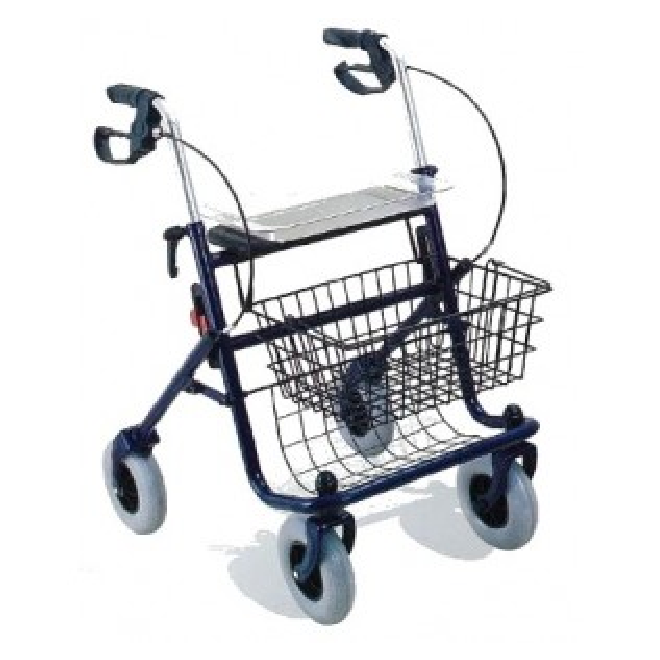
\includegraphics[width=0.45\columnwidth]{images/rollator.eps}
	\caption{A 4 wheeled rollator}
	\label{fig:rollator}
\end{figure}

Rollators induce a more natural gait pattern than standard four legged frames. They are designed for people that need less weight bearing~\cite{VanHook03}.

\subsection{Existing smart rollators}

Here is an overview of the the existing smart rollators, focusing on common wheeled walker that connects to a person at the hands. Smart walkers may be used to analyse either the environment or  the user's behaviour. Environmental data is dedicated to navigation purpose, such as obstacle avoidance~\cite{Spenko06}, wall following~\cite{Yu2003}, slope compensation~\cite{Hirata2007} or localisation~\cite{Kotani1996,MacNamara00}. Even though these functionalities are relevant for people autonomy, especially for the visually impaired, these functionalities are out of the scope of this paper that focuses on gait analyses. A thorough survey on assistance mobility device, focusing on smart walkers can be found in~\cite{Frizera08,Martins11}.\\

Some of the existing Smarts walkers aim at tracking the trajectories of gait features in order to monitor health. The great advantage of such systems is that the user stands at a roughly known position with regards to the walker. Body segment localisation is then made easier.

Walkers can be equipped with force-moment sensors mounted on the walker handles~\cite{Alwan07,Tung10}, or under the forearm~\cite{Frizera08,Frizera10b} to passively derive some gait characteristics. In both cases it is assumed that the force and moment recorded have cyclic changes reflecting the gait cycle and that these changes depend on basic gait features (cadence, stride time, gait phases).  The iWalker ~\cite{Tung10} quantifies loads exerted through the handles an frame and standards spatio-temporal parameters (such as speed and distance). In~\cite{Alwan07}, a direct comparison between motion capture and force-moment data was studied to detect significant pattern in the force signal. The lateral sway motion of the upper body reflects in peaks in vertical direction and in the corresponding forward moment signal. These peaks coincided with the heel initial contacts and. The forward propulsion force applied by the user is related to the toe-off event from the right and left toe. Finally, the stride (ie. duration of a gait cycle) can be computed from two heel contacts. In~\cite{Frizera10b}, a method based on Weighted Frequency Fourier Linear Combiner, is introduced for the same standards gait parameters extraction from force data.

Walker wheel motion measurement can also be used to estimated the user state~\cite{Spenko06,Merlet10b}. The Personal aid for mobility and monitoring project (PAMM)~\cite{Spenko06} developed health monitoring tools. The PAMM smart walker is an omnidirectional walker design for walking assistance with navigation and monitoring functionalities. Its sensors record user speed and compute the stride-to-stride variability, which have been shown to be an effective predictor of falls. A power spectrum analysis on PAMM's velocity allows to estimate user's stride length and frequency. Besides, the shape of the power spectrum is related to the gait symmetry. Indeed, for a symmetric gait, the energy is located at twice the stride frequency. However, the system can detect asymmetric gait as spectrum with energy located at the stride frequency and at higher frequency. An asymmetrical gait could be an indicator of a physical injury or a minor stroke.

Direct measurement of body segments may be obtained by using ultrasonics sensors or cameras \cite{Frizera08,Chee09}. A vector of ultrasonic sensors can be mounted on the walker to scan the space between the user and the walker and determine coordinate of each leg without adding any marker on the patient~\cite{Frizera08}. In ~\cite{Chee09}, a camera is mounted on the frame and observes markers on the toes. This marker based toe tracking algorithm allows to calculate step width and provide an accurate assessment of foot placement during rollator use.
  
The main issue when using that kind of device is that the accuracy of the leg localisation depends strongly on the clothes that the user wears. It is a drawback with regards to method based on odometers or force sensors. The method proposes in~\cite{Chee09} by-passes this point by adding markers on the toes. Yet it also by-passes our constraint not to equip the user in order to ensure acceptance and ease of use.

Extrinsic data can then be used to monitor the user's health or to control the walker in order to prevent a fall. The walker-user relative distance can be used to classify the states between a \textit{walking state}, a \textit{stopped state }and an \textit{emergency state} \cite{Hirata2006}. A laser range finder mounted on the walker acquired the position of the knee with regards to the walker frame. It is assumed that the position of the feet is at the vertical of the knee position, and fixing the human frame in the middle of the feet. User velocity is estimated from the walker velocity obtained by odometers. The\textit{ stopped state} occurs when both the walker and the human velocities are null. To distinguish the \textit{walking state} from the \textit{emergency state}, user-walker distance is used.  A normal distance distribution is computed to determine the  \textit{walking state} based on user data. The robot control tries to bring the user distance right to the mean of the  walking state distance distribution.

In~\cite{Hirata2008a} the RT-Walker is equipped with laser range finder and perform an estimation of the kinematics of a 7-link human model. The model is used to estimate the position of the user center of gravity (CoG) in 3D. A stable region is determined by analysing the distribution of the C.o.G. position for three subjects with different physiques who walked for 100 seconds with a walker. If the C.o.G is out of the region, the user may fall. The system then brakes enough to compensates for its lightweight and prevent the fall. Notice that the fall detection is restricted to the sagital plane.

In~\cite{Taghvaei10}, The RT Walker is equipped with vision sensor to classify the user state among four classes : sitting, standing, falling, and walking. The classifier is based on heuristic on the distance between user head, hands and shoulder. Basically, the vision algorithms are based on head tracking, and skin detection. Shoulder detection is performed by finding the higher points of a uniform color region under the head, which seems to lack robustness with regards to environment properties and user clothes.   

%Monitoring systems allow to estimate biomechanical features in ambulatory conditions, i.e. in uncontrolled conditions. Information about the walker itself (odometry, inertial parameters) or user-walker interaction seems more robust in these condition than laser data, video or distance sensors because they do not rely on environmental parameters such as user clothes and lightning condition. Yet, these sensors can provide useful and complementary information about user posture.

%Walking assistance based on user intend allows to control the direction of the walker. Fall prevention algorithm tend to draw the boundaries between "normal situations" and "risk of fall". Most of the time, the control strategy consists in braking to stop the system.
\subsection{Our smart rollator}

In this paper, the system aims at tracking some specific parameters for biomechanical gait analysis, that were chosen in \cite{Dune2012}: 
\begin{itemize}
\item step length
\item step width
\item step frequency
\item feet orientation
\item heel trajectory
\item ankle angle trajectory
\end{itemize}

\begin{figure}[h]
	\centering
	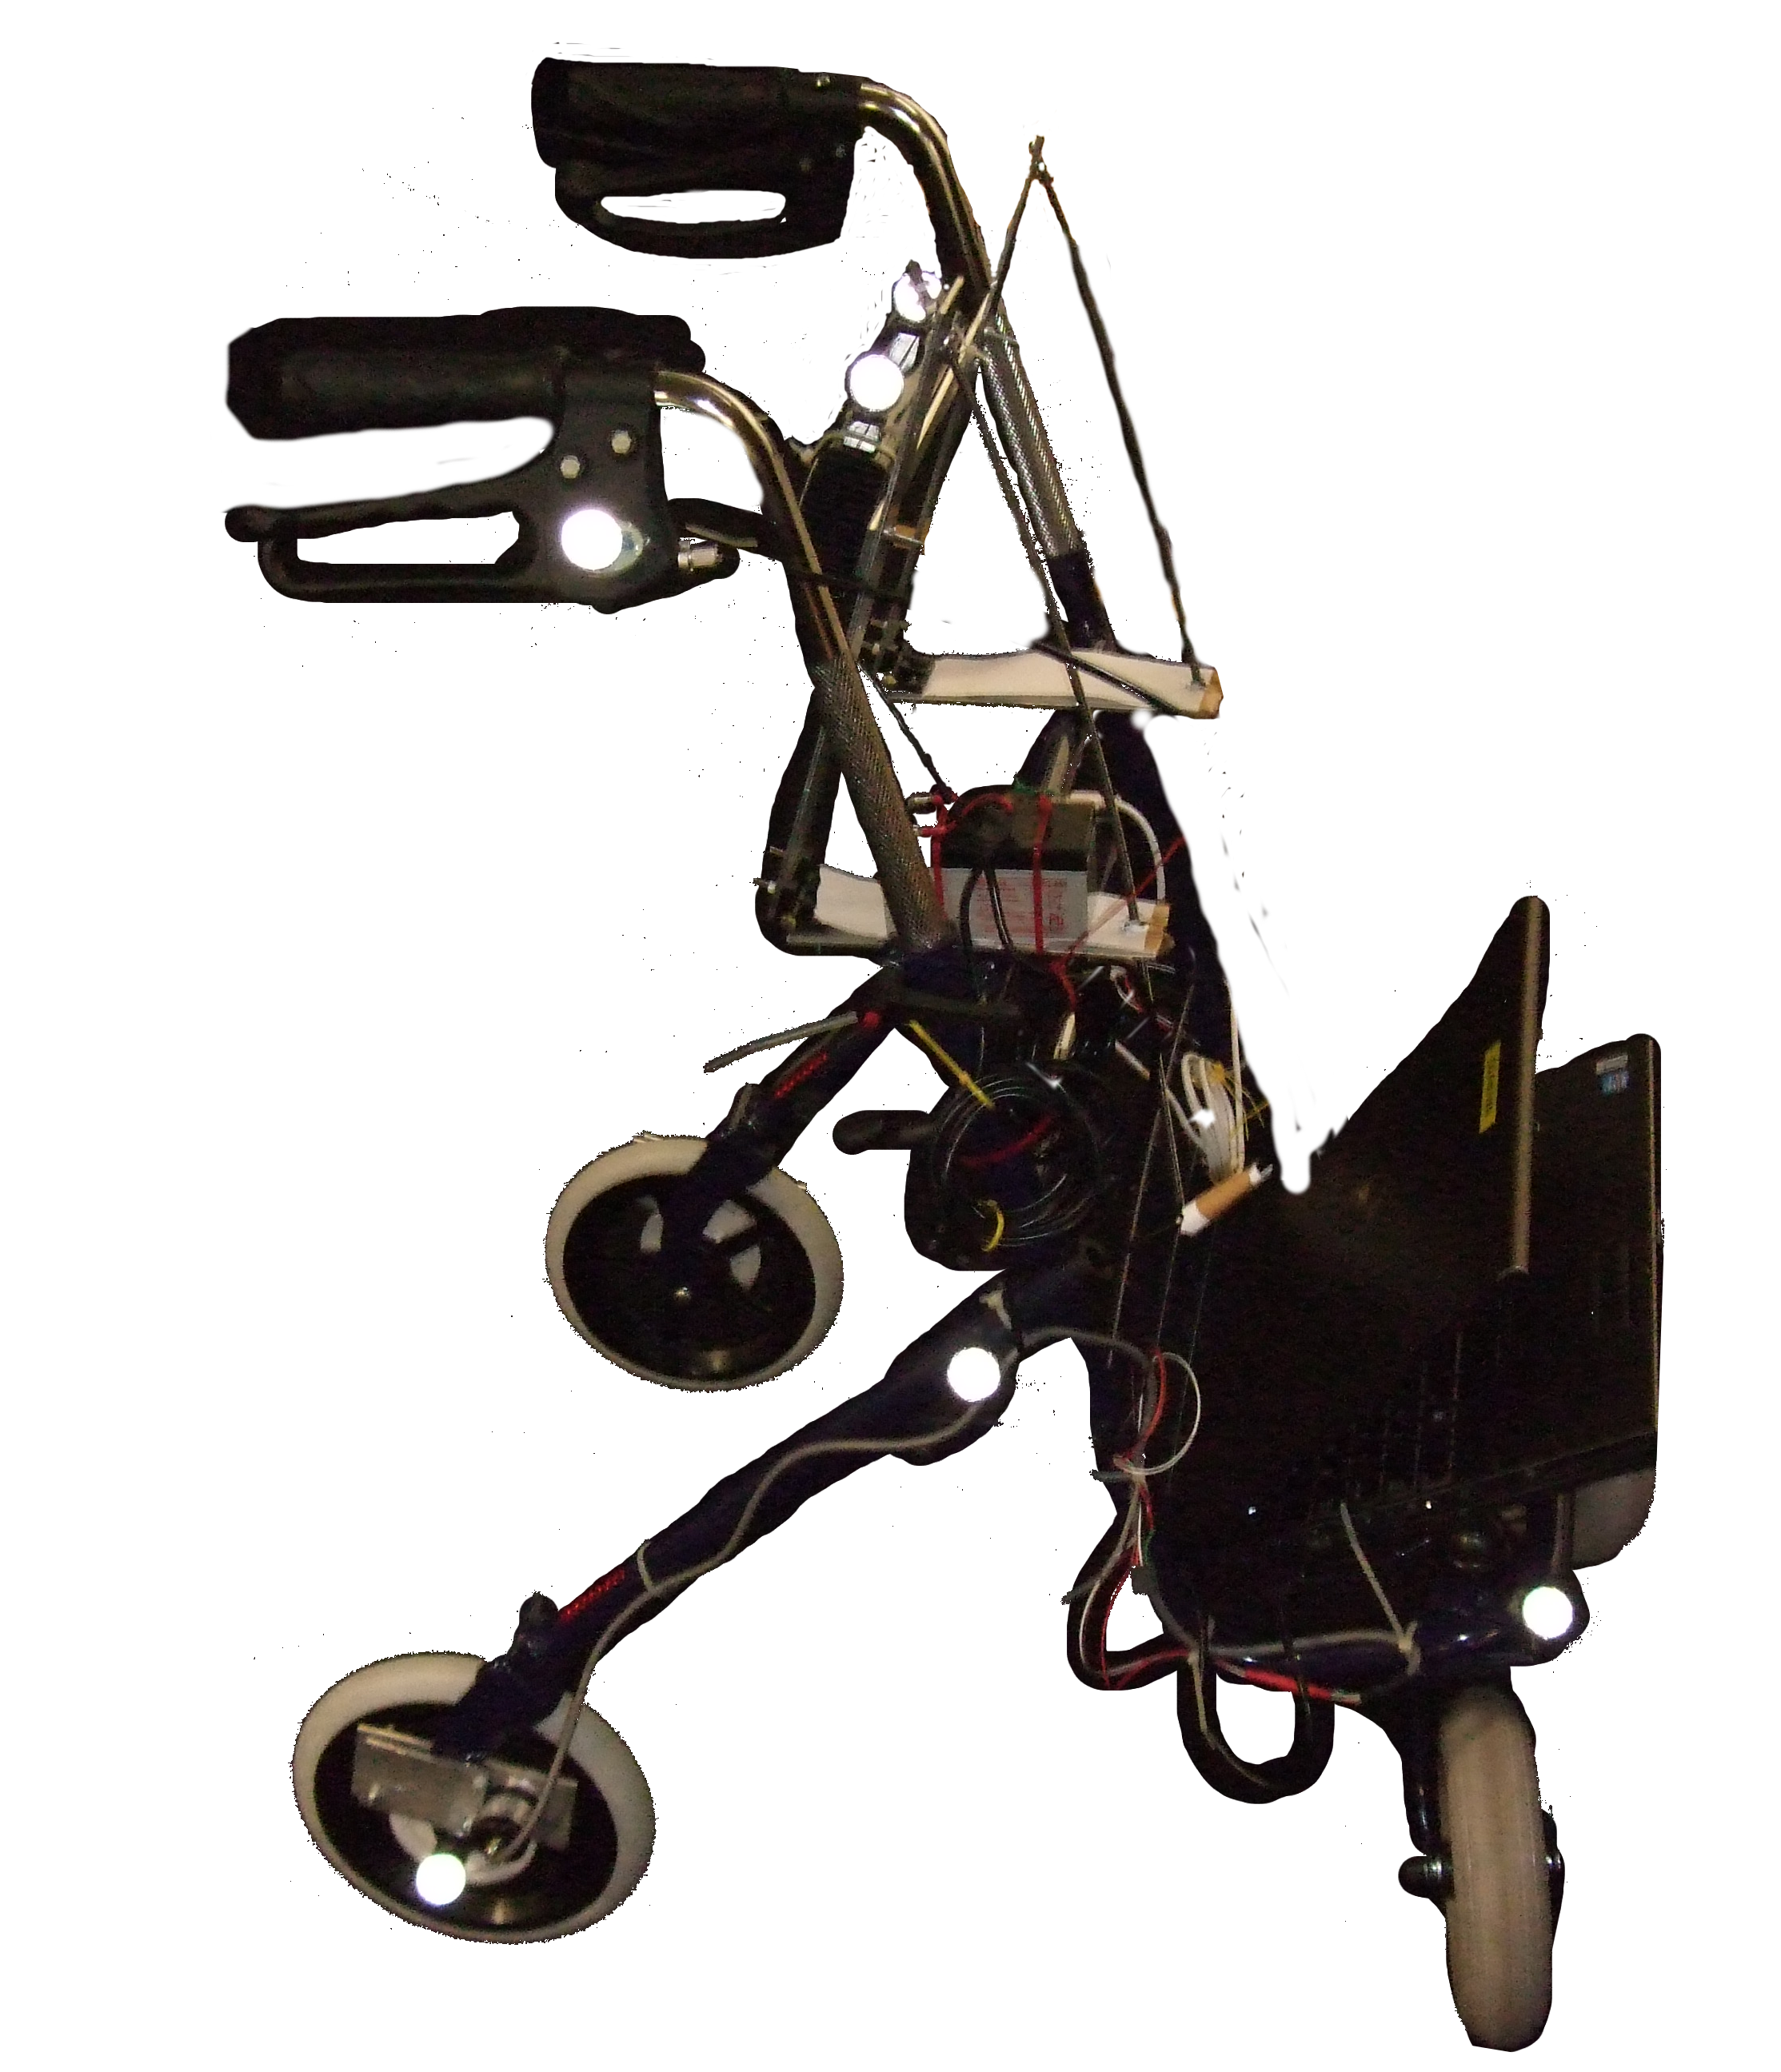
\includegraphics[width=0.45\columnwidth]{images/ourRollator.eps}
	\caption{Our smart rollator : a 4 wheeled rollator equipped with odometers and a kinect sensor}
	\label{fig:ourrollator}
\end{figure}


Our system is made \CD{of}{by} a standard \CD{4 wheeled rollator}{walker} \CD{equipped with sensors}{on which some equipment was installed} (fig.~\ref{fig:ourrollator}):
\begin{itemize}
	\item The Kinect sensor which is viewing the feet of the person.
	\item Odometers \CD{are}{were} mounted on the rear wheels to estimate the trajectory of the walker.
	\item A laptop \CD{is}{was} installed to grab the sensor data
	\item Finally, motion capture\footnote{A Qualysis system is used.} markers \CD{are}{were} installed in order to compute the ground truth. 
\end{itemize}


In this paper, we focus on the estimation of leg and feet poses in a Frame attached to the Kinect sensor. With such data, some interesting parameters like feet orientation or ankle angle trajectory can be directly computed. This is the main topic of this paper. Computation of step length and width may be done by fusing the results of this paper with odometry (out of scope here). \CD{This could be done by integrating the robot motion to computes its pose in a fixed reference frame. Then, the current feet pose could be directly expressed in this fixed reference frame to compute the step length and width.}{}



\section{Algorithm for Kinect processing}
\label{sec:Algorithm}

\begin{figure}
	\centering
	\includegraphics[width=0.45\textwidth,trim=4cm 2cm 2cm 3cm,clip=true]{images/KinectFrames}
	\caption{Left: kinect depth map. The warmer is the color, the larger the depth associated is -- Right: 3D points cloud associated to the depth map (for clarity the feet, rollator and ground were segmented).}
	\label{fig:KinectFrames}
\end{figure}

The algorithm to process Kinect images is presented in this section. \CD{The method aims at fitting a 3D skeleton on the partial kinect data. The 2 legs will be described as two rigid bodies linked with a ball joint (which represent an approximation of the ankle joint).}{The goal of the method is to segment  Kinect points cloud (see Fig.~\ref{KinectFrames}) in two part (left and right) which are composed by}:

\begin{itemize}
	\item a first segment which links the toe to the heel
	\item a second segment which has a predefined length starting from the heel in the direction of the leg
\end{itemize}
\CD{To do so}{Moreover}, a \CD{parametric}{} model will be \CD{fitted}{fit} to each feet and leg. This will be done in four steps:
\begin{enumerate}
	\item The first step consists in removing from Kinect \CD{depth maps}{images} the points associated to the ground and those associated to the rollator,
	\item The second step consists in making a first segmentation of the feet and legs thanks to a model based method. The model used corresponds to a cylinder (legs) and a plane (feet)
	\item The third step consists in optimizing the former segmentation and the model parameters by optimizing both legs and feet model simultaneously, eg. by taking into account the fact that the two legs have the same diameter.
	\item Finally, the last step consists in transforming the former 2 body model introduced before. This model will be used as measurements in a Kalman filter (see section~\ref{sec:Kalman}).
\end{enumerate}
We propose to describe these four steps in the following paragraphs.

\subsection{Ground and walker segmentation}
\label{subsec:GroundWalkerSeg}
In our experiments, the walker is used indoors on a flat ground. Since the Kinect sensor is rigidly fixed to the walker, the ground plane will be the same in all images. As a consequence it is possible to compute it once and for all and to consider it as constant. An other solution could consists in detecting the main plane of the 3D points cloud with a RANSAC algortithm. \CD{The orientation of the kinect with regards to the ground plane can be used to compute the position of the point in a frame align with the ground. It eases the reading of the point cloud.}{Moreover, a rotation matrix can be defined in order to change its orientation to an horizontal plane. At this step, we assume that the we apply this rotation matrix so that the $\mathbf{z}$ axis in the Kinect frame corresponds to the $\mathbf{z}$ axis of the world}.

The rollator does not move with respect to the Kinect and so is static in the Kinect camera frame. It can be removed from the depth map by using a predefined mask.

In the following, we defined by $\Omega$ the set of the points which do not belong neither to the ground nor to the rollator. 


\subsection{Feet and legs segmentation}

The main idea of feet and legs segmentation is based on region growing and inspired by \cite{aaa}. From a current set of points of a member, we look for potential candidates in the neighbouring and then validate it or not. The following paragraphs are dedicated to the presentation of the process. The global algorithm is presented in paragraph~\ref{subsub:generalAlgo}. Then application for legs and feet segmentation is presented (paragraph~\ref{subsub:legSegmentation} and~\ref{subsub:footSegmentation}).

\subsubsection{General algorithm}~\\
\label{subsub:generalAlgo}
The general algorithm for member (a foot or a leg) segmentation is presented here:
\begin{enumerate}
	\item Let $\mathcal{M}$ be the set of the current image points belonging to the member and $\mathbf{p}$ a \textbf{set of parameters} associated to it
	\item Let $\mathcal{N}$ be the set of neighbours associated to $\mathcal{M}$:
	\begin{equation}
		\mathcal{N} = \{\mathbf{n}\notin\mathcal{M}\ |\ \exists \mathbf{m}\in\mathcal{M}, \|\mathbf{n} - \mathbf{m}\| \leq s \}
		\label{eq:defV}
	\end{equation}
	where $s$ is a threshold to define (8-10 pixels). Note that in \eqref{eq:defV} $\mathbf{m}$ and $\mathbf{v}$ are not 3D points but pixels in Kinect image.
	\item $\mathcal{N}$ represents the set of new potential candidates. We remove from this set all the points that belongs to the ground or to the walker. Moreover, the points that do not match enough with the current model defined by $\mathbf{p}$ are also removed. Thus, the final candidates are defined by:
	\begin{equation}
		\mathcal{N}' = \{\mathbf{n}\in\mathcal{N}\ |\ \mathrm{dist(\mathbf{n},\mathbf{p})}\leq s^{pts}\}\cap\Omega
	\end{equation}
	where $\mathrm{dist}$ is the function which gives the distance of a point (first argument) to a model (second argument), $s^{pts}$ a threshold and $\Omega$ the set defined in \ref{subsec:GroundWalkerSeg}.
	\item 2 cases can be distinguished:
	\begin{enumerate}
		\item $\mathcal{N}'=\emptyset$: there is not any new candidate. The set of points associated to the member is complete. The set $\mathcal{M}$ and the last set of parameters computed $\mathbf{p}$ are returned.
		\item $\mathcal{N}'\neq\emptyset$: in this case, there are new points to add to the model. A new model $\mathbf{p'}$ is computed with the point set:
		\begin{equation}
			\mathbf{p'} = \mathrm{fit}\left(\mathcal{M}\cup\mathcal{N}'\right)
		\end{equation}
		where $\mathrm{fit}$ is the function that computes a model by fitting the 3D points associated to the set given in argument.
	\end{enumerate}
	\item The new model $\mathbf{p'}$ is then tested by comparing the mean error to a threshold $s^{mod}$:
	\begin{equation}
		\mu = \frac{1}{\mathrm{card}\left(\mathcal{M}\cup\mathcal{V}'\right)}\cdot
		\sum_{\mathbf{m}_{i}\in\left(\mathcal{M}\cup\mathcal{V}'\right)} \mathrm{dist}(\mathbf{m}_i,\mathbf{p})
	\end{equation}
	2 cases can be distinguished:
	\begin{enumerate}
		\item $\mu > s^{mod}$: the mean error with the new model is too important and so it is rejected. The new points $\mathcal{N}'$ are discarded. The algorithm terminates and returns the set $\mathcal{M}$ and the parameters $\mathbf{p}$.
		\item $\mu < s^{mod}$: the new model is accepted with the complete set of points. We return to \textbf{step 1} to make it grow again with the following parameters:
		\begin{eqnarray}
			\mathcal{M}&\leftarrow&\mathcal{M}\cup\mathcal{N}'\\
			\mathbf{p} &\leftarrow& \mathbf{p}'
		\end{eqnarray}
	\end{enumerate}
\end{enumerate}

\subsubsection{Leg segmentation}~\\
\label{subsub:legSegmentation}

\paragraph{Model and definition of $\mathrm{dist}$ function}~\\
\label{paragraph:paramCylindre}
To segment the legs, a \emph{cylinder model} is used. It is a 5 parameters primitive (4 parameters stand for its axis and one for its radius). The distance considered is the radial distance to the cylinder.  Let $\mathbf{m}$ be a Kinect image point whose distance to the cylinder of parameters $\mathbf{p}$ has to be evaluated. It is computed with the following steps:
\begin{enumerate}
	\item Let $\mathcal{B}=(\mathbf{u},\mathbf{v},\mathbf{w})$ be an orthnormal base with $\mathbf{w}$ in the same direction than the cylinder axis and  $\mathbf{C}$ a point belonging to this axis. The rotation matrix $\mathbf{R}$  $(\mathbf{x},\mathbf{y},\mathbf{z})$ initiale à $\mathcal{B}$:
	\begin{equation}
		\mathbf{R} = 
		\begin{bmatrix}
			\mathbf{u} & \mathbf{v} & \mathbf{w}
		\end{bmatrix}
	\end{equation}
	\item Let $\mathbf{M}$ be the 3D point (in the Kinect frame) associated to $\mathbf{m}$ and $\mathbf{M}'$ the coordinates of $M$ in the frame defined by $(\mathbf{C},\mathcal{B})$:
	\begin{equation}
		\mathbf{M}' = \mathbf{R}\left(\mathbf{M}-\mathbf{C}\right)
	\end{equation}
	Finally, the distance to the cylinder is the difference between its radius (noted $a$ in the following) and the distance between $\mathbf{C}$ and the projection of $\mathbf{M}'$ in the plane $(\mathbf{C},\mathbf{u},\mathbf{v})$. With $\mathbf{M}'=[x\ y\ z]^T$, we have:
	\begin{equation}
		\mathrm{dist}(\mathbf{m},\mathbf{p}) = |\sqrt{x^2+y^2} - a|
	\end{equation}
	where $\mathbf{p}$ stands for the cylinder parameters (see paragraph~\ref{subsub:paramCylindre}) and are used to define $\mathbf{u}$, $\mathbf{v}$, $\mathbf{w}$, $\mathbf{R}$, $\mathbf{C}$ and $a$.
\end{enumerate}

\paragraph{Model parameterization}:~\\
A cylinder can be defined by the rotation matrix $\mathbf{R}$,the point $\mathbf{C}$ and its radius $a$ which were introduced in the previous paragraph. A rotation matrix has 3 degrees of freedom and can be written has the multiplication of 3 matrices:
\begin{equation}
	\mathbf{R} = \mathbf{R_3}(\theta_3)\cdot\mathbf{R_2}(\theta_2)\cdot\mathbf{R_1}(\theta_1)
	\label{eq:defR}
\end{equation}
where $\mathbf{R_1}(\theta_1)$ (resp. $\mathbf{R_2}(\theta_2)$, $\mathbf{R_3}(\theta_3)$) stand for the rotation matrix around the first (resp. second, third) canonical axis of angle $\theta_1$ (resp. $\theta_2$, $\theta_3$). $\mathbf{C}$ can be defined by 3 coordinates:
\begin{equation}
	\mathbf{C} = \begin{bmatrix}
			c_x & c_y & c_z
		\end{bmatrix}^T
	\label{eq:defC}
\end{equation}
From \eqref{eq:defR} and \eqref{eq:defC}, cylinder pose uses 6 parameters. However, it is possible to use only 4 parameters. Using 6 parameters could lead to divergence during optimization. We propose to use only 4 parameters by using the following remarks: 
\begin{enumerate}
	\item Since a cylinder has a revolution symmetry, there is an infinite number of solution to define the base $(\mathbf{u},\mathbf{v},\mathbf{w})$. Only the direction of $\mathbf{w}$ is important (it corresponds to the direction of the cylinder); as a consequence, any rotation of $(\mathbf{u},\mathbf{v})$ around $\mathbf{w}$ can change the results of distance computation. So, we can multiply by the left the matrix $\mathbf{R}$ by any matrix of the form $\mathbf{R_3}(\theta)$ ($\theta\in[0\ 2\pi]$) without modifying the function $\mathrm{dist}$. As a consequence, any value of $theta_3$ is valid. So, we chose to fix it to zero and do not estimate it.
	\item Finally, the choice of $\mathbf{C}$ is not unique: every point of the cylinder axis is valid. Thus, there is one degree of freedom to remove. To do it and force they unicity of $\mathbf{C}$, it was chosen to fix the third component ($c_z$, see~\eqref{eq:defC}). Fixing this component is save as soon as the cylinder axis is not perpendicular to the $\mathbf{z}$ axis.\footnote{Which corresponds to the direction perpendicular to the ground, see paragraph~\ref{}} Such situation implies that the leg is parallel to the ground, which does appear in our context. So, parameters $c_x$ and $c_y$ can be seen as a function of $c_z$ which is arbitrarily \footnote{Not really in practice. $c_z$ is chosen so that it is possible to find a good initialisation of $c_x$ and $c_y$ to optimize the minimisation process during fitting.}
\end{enumerate}

Finally, each leg is represented by a cylinder which parameters are stored in a 5D vector:
\begin{equation}
	\mathbf{p} = \begin{bmatrix}
		c_x & c_y & \theta_1 & \theta_2 & a
	\end{bmatrix}^T	
\end{equation}
This representation ensure that there is one and only one possibility to define the point $\mathbf{C}$ and the rotation matrix $\mathbf{R}$.


\paragraph{Definition of $\mathrm{fit}$ function}~\\
The $\mathrm{fit}$ function aims to estimate a vector parameters $\mathbf{p}$ associated to a set of Kinect points $\mathcal{M}$. Soit $\mathbf{f}(\mathcal{M},\mathbf{p})$ the vector defined by:
\begin{equation}
	\mathbf{f}(\mathcal{M},\mathbf{p}) = \frac{1}{1+\e^{-a}}\cdot
	\begin{bmatrix}
		\mathrm{dist}(\mathbf{m}_1,\mathbf{p}) \\
		\vdots \\
		\mathrm{dist}(\mathbf{m}_N,\mathbf{p})
	\end{bmatrix}
	\label{eq:defEstCyl1}
\end{equation}
with $\mathcal{M} = \{\mathbf{m}_i,i\in[1\dots N]\}$.
$\mathrm{fit}$ is then defined by:
\begin{multline}
	\mathrm{fit}(\mathcal{M}) = 
	\min_{\mathbf{p}}
	\left(
		\left(\mathbf{f}(\mathcal{M},\mathbf{p})\right)^T\cdot
		\left(\mathbf{f}(\mathcal{M},\mathbf{p})\right)
	\right) \\=
	\min_{\mathbf{p}}
	\left(
		\left(1+\e^{-a}\right)^{-2}\cdot\sum_{\mathbf{m}_i\in\mathcal{M}} \mathrm{dist}^2(\mathbf{m}_i,\mathbf{p})
	\right)
	\label{eq:defEstCyl2}
\end{multline}
In~\eqref{eq:defEstCyl2}, the minimum is computed with the Levenberg-Marquardt method. Initial conditions are fixed as follows:
\begin{enumerate}
	\item $c_x$ and $c_y$ are initialized with the barycenter of the 3D points cloud. The value of $c_z$ is then \emph{fixed} as the mean of the $z$ coordinates associated to the 3D points cloud ($z$ is not modified during the minimization process).
	\item $\theta_1$ and $\theta_2$ are provided thanks to the covariance matrix associated to the 3D points cloud. The axis cylinder $\mathbf{w}$ is assumed to be equal to the eigen vector associated to the largest eigen value (since the length of the leg is larger than the radius cylinder). The parameters $\theta_1$ and $\theta_2$ can the be easily computed.
	\item $a$ is initialized to 0.05m.
\end{enumerate}
\begin{rem}
In \eqref{eq:defEstCyl1} and \eqref{eq:defEstCyl2}, $(1+\e^{-a})^{-1}$ is used to penalize solutions with a large radius. Since the 3D points cloud associated to the legs corresponds only to a partial cylinder (around 30deg), the radius is not easily observable and the function to minimize tends to be ``plate''. Introducing $(1+\e^{-a})^{-1}$ yields in slightly favoring cylinder with smaller radius. Moreover, it can be obserbed that $(1+\e^{-a})^{-1}$ is always between $1$ and $1/2$ and can not have a strong influence on the final result or make converge the final result to a radius close to zero.\footnote{This is not be the case with a factor such as $\sqrt{a}$ like in \cite{lala}.}
\end{rem}
\subsubsection{Foot segmentation}~\\
\label{subsub:footSegmentation}
\paragraph{Model and definition of $\mathrm{dist}$ function}~\\
For the feet, a planar model is used and is parameterized by its 4 equation parameters:
\begin{equation}
	\left\{
	\begin{array}{l}
		\mathbf{p} = 
		\begin{bmatrix}
			a & b & c & d
		\end{bmatrix}^T\\
	\mbox{avec } |\mathbf{p}\| = 1 
	\end{array}
	\right.
\end{equation}
so that every 3D points $[x\ y\ z]^T$ belong to the plane verify:
\begin{equation}
	ax+by+cz+d=0
\end{equation}

The function $\mathrm{dist}$ corresponds to the Euclidean distance to the plane. Let $\mathbf{m}$ be an image point associated to the foot and $\mathbf{M} = [x\ y \ z]^T$ the 3D point associated to it:
\begin{equation}
	\mathrm{dist}(\mathbf{m},\mathbf{p}) = 
	\frac{|ax+by+cz+d|}
	{\sqrt{a^2+b^2+c^2}}
\end{equation}


\subsubsection{Definition of $\mathrm{fit}$ function}~\\

The $\mathrm{fit}$ function is defined as the minimization of the error function to the plane with the constraint $\|\mathbf{p}\|=1$. Let $\mathcal{M}$ be the set to fit and $\mathbf{g}(\mathcal{M},\mathbf{p})$ the vector defined by:
\begin{equation}
\mathbf{g}(\mathcal{M},\mathbf{p})=
	\begin{bmatrix}
		ax_1 + by_1 + cz_1 +d \\
		\vdots\\
		ax_N + by_N + cz_N + d
	\end{bmatrix}
	\label{eq:defEstPlan1}
\end{equation}
with:
\begin{equation}
	\left\{
		\begin{array}{l}
			\mathcal{M} = \{\mathbf{m}_i,i\in[1\dots N]\}\\
			\{\mathbf{M}_i,i\in[1\dots N]\}\mbox{the 3D points associated to }\mathcal{M}\\
			\forall i\in[1\dots N],\ \mathbf{M}_i = \begin{bmatrix} x_i & y_i & z_i \end{bmatrix}^T
		\end{array}
	\right.
\end{equation}
So we have:
\begin{equation}
	\mathrm{fit}(\mathcal{M}) = \min_{\mathbf{p}\in\mathbb{R}^4,\ \|\mathbf{p}\|=1}\left(\left(\mathbf{g}(\mathcal{M},\mathbf{p})\right)^T\left(\mathbf{g}(\mathcal{M},\mathbf{p})\right)\right)
	\label{eq:defEstPlan2}
\end{equation}
\eqref{eq:defEstPlan2} can be exactly solved with Lagrange multiplier method. Let $\mathbf{A}$ be the matrix defined by:
\begin{equation}
	\mathbf{A}=
	\begin{bmatrix}
		x_1 & y_1 & z_1 & 1 \\
		\vdots & \vdots & \vdots & \vdots \\
		x_N & y_N & z_N & 1 \\
	\end{bmatrix}
\end{equation}
We have:
\begin{equation}
	\mathrm{fit}(\mathcal{M}) = \mathbf{vp}(\mathbf{A}^T\mathbf{A},1)
	\label{eq:defEstPlan3}
\end{equation}
where  $\mathbf{vp}(\mathbf{X},i)$ stands for the normalized eigen vector associated to the i-th  eigen value of $\mathbf{X}$ (In~\eqref{eq:defEstPlan3}, it corresponds to the smallest eigen value).

\subsubsection{Initialization of the set}~\\
The global method proposed to segment the feet and the legs needs to provide an initial set of image points for each member. This is done by the following steps and illustrated on Fig.~\ref{fig:segmentation}~:
\begin{enumerate}
	\item Firstly, it can be noticed that after removing the ground and the rollator from the Kinect image, there are two ``big'' sets of points that can be easily segmented and corresponding to the left and right member (Fig.~\ref{subfig:seg1}). If there are other small sets due to noise, they can thus be discarded.
	\item Then each part contains both the foot and the leg. Because of the geometry of the system, the bottom part corresponds systematically to the leg. Thus, we chose to initialize the leg with the last bottom quarter and the foot with the first bottom quarter (Fig.~\ref{subfig:seg2})
	\item Finally, the algorithm makes grow these sets, thus computing the final segmentation (Fig.~\ref{subfig:seg3}).
\end{enumerate}
\begin{figure*}
	\centering
	\subfloat[][After ground and rollator segmentation]{\label{subfig:seg1}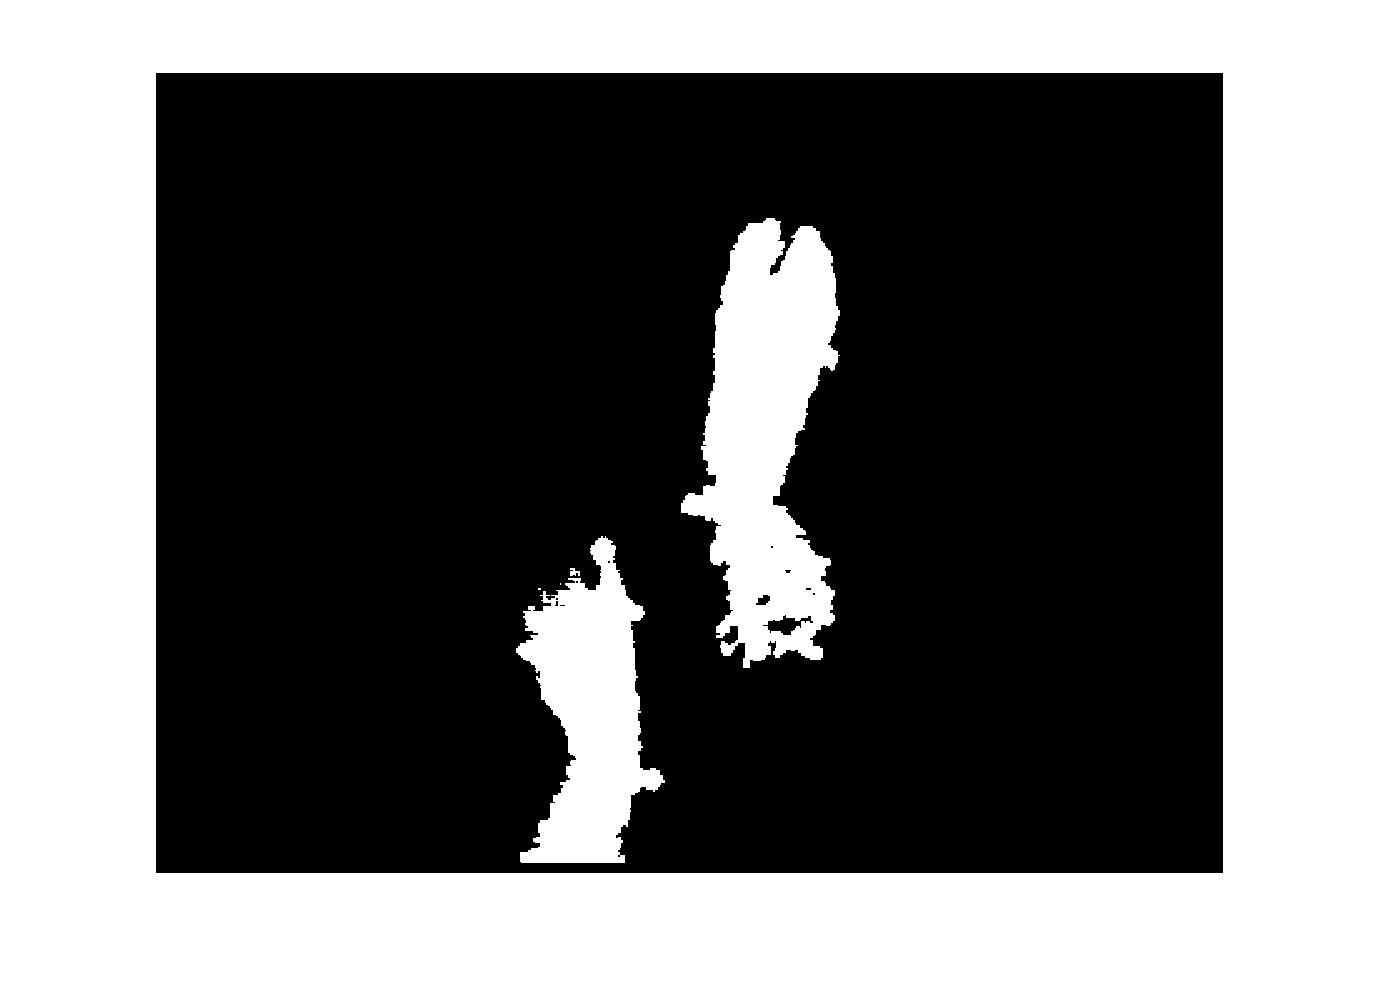
\includegraphics[width=0.32\textwidth]{images/seg0}}\hfill
	\subfloat[][At initialization)]{\label{subfig:seg2}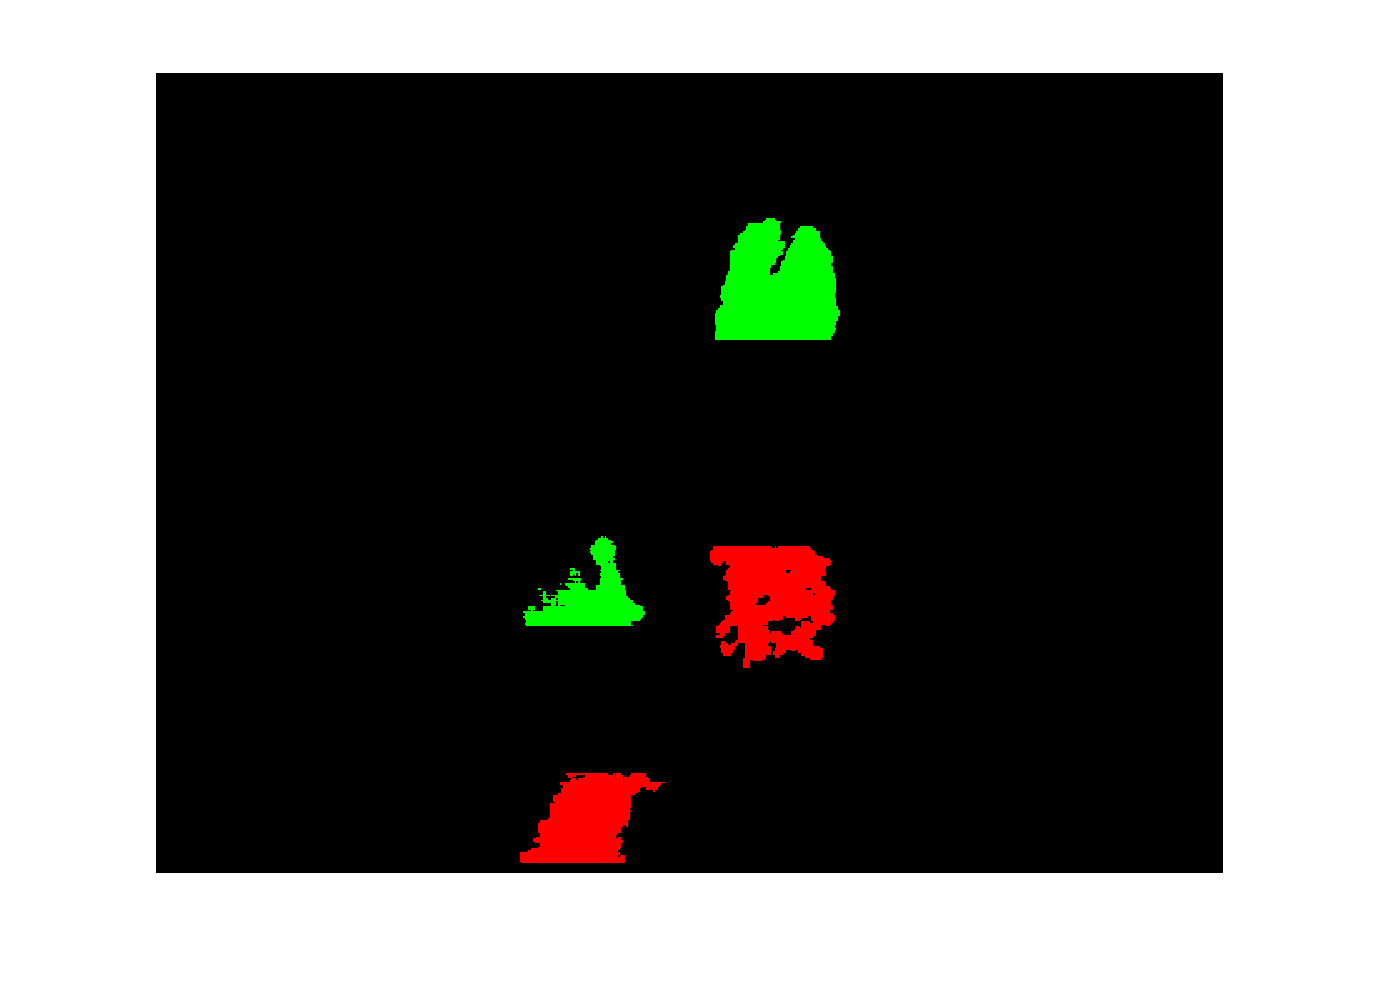
\includegraphics[width=0.32\textwidth]{images/segIni}} \hfill
	\subfloat[][Final result)]{\label{subfig:seg3}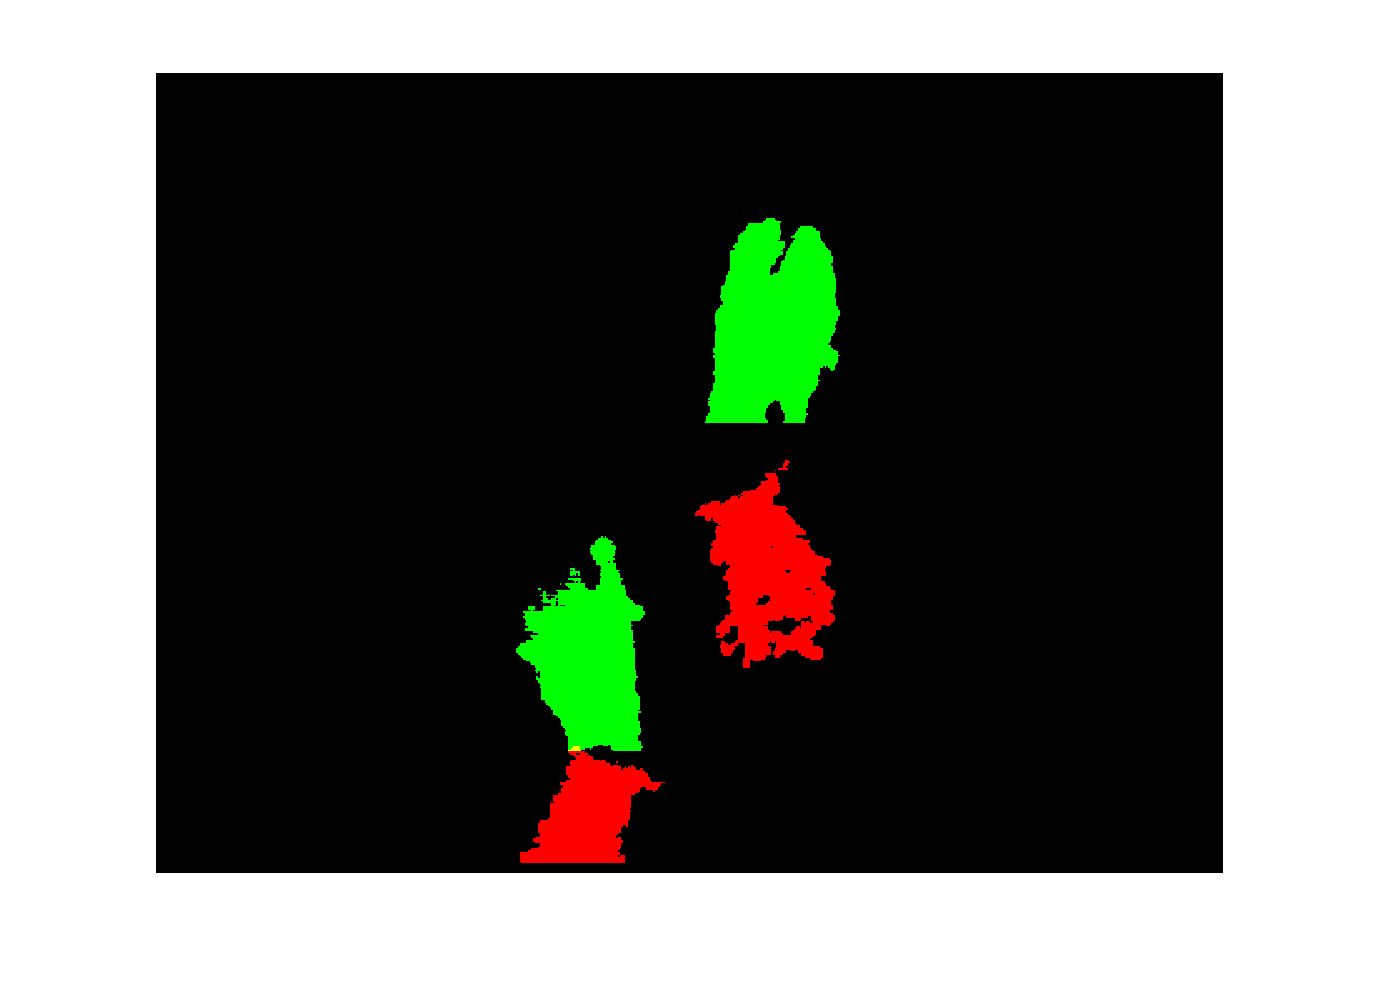
\includegraphics[width=0.32\textwidth]{images/segEnd}}
	\caption{Steps of segmentation}
	\label{fig:segmentation}
\end{figure*}

\subsection{Model optimization}
After the segmentation step, a model has been computed for each member. We propose now to optimize these parameters.

\subsubsection{Legs}~\\
In the following, the two legs will be {optimized simultaneously}. During the segmentation step, they were optimized independently. So, it was guaranteed that both legs have the same radius. At this step, we propose to estimate both parameters from the 3D points extracted from the segmentation with the constraints that they have the same radius. So, we define a new vector to optimize:
\begin{equation}
	\mathbf{p_{legs}} = 
	\begin{bmatrix}
		c_x^g & c_y^g & \theta_1^g & \theta_2^g & c_x^d & c_y^d & \theta_1^d & \theta_2^d & a
	\end{bmatrix}^T
\end{equation}
where:
\begin{itemize}
	\item $c_x^l$, $c_y^l$, $\theta_1^l$ and $\theta_2^l$ stand for the parameters defining the pose of the cylinder associated to the left leg,
	\item $c_x^r$, $c_y^r$, $\theta_1^r$ and $\theta_2^r$ stand for the parameters defining the pose of the cylinder associated to the right leg.
\end{itemize}
Thus, the whole points are fitted in the same optimization process (of course, each point is labeled with its own leg). The methods is roughly the same that during segmentation. Nevertheless, it is interesting to note that the new Jacobian matrix has a block structure with two zero blocks.

\paragraph{Feet}~\\
Finally, the sets associated to the feet are optimized by using stronger thresholds in order to remove outliers.

\subsection{Final parameters}
The final step consists in transforming the legs and feet parameters into a bone representation. For each side, we have:
\begin{enumerate}
	\item The heel is computed as the intersection between the axis cylinder and the plane associated to the foot. More precisely, since the plane corresponds to the \emph{top of the foot}, it does not correspond exactly to a point which is higher. Then, a segment starting from this point in the direction of the leg is defined to visualize the leg.
	\item The toe we get it by using the foot plane and the 3D points associated. It is computed in steps:
	\begin{enumerate}
		\item Firstly, the 3D point cloud is projected onto the plane computed previously
		\item Then, the convex hull of this projection is computed with its barycenter.
		\item The vector joining the ``hell'' to this barycenter provides the foot direction. The further 3D point in this direction define the toe.
	\end{enumerate}
\end{enumerate}
An example of the results provided by the algorithm is provided on fig.~\ref{fig:exampleBones}

\begin{figure}
	\centering
	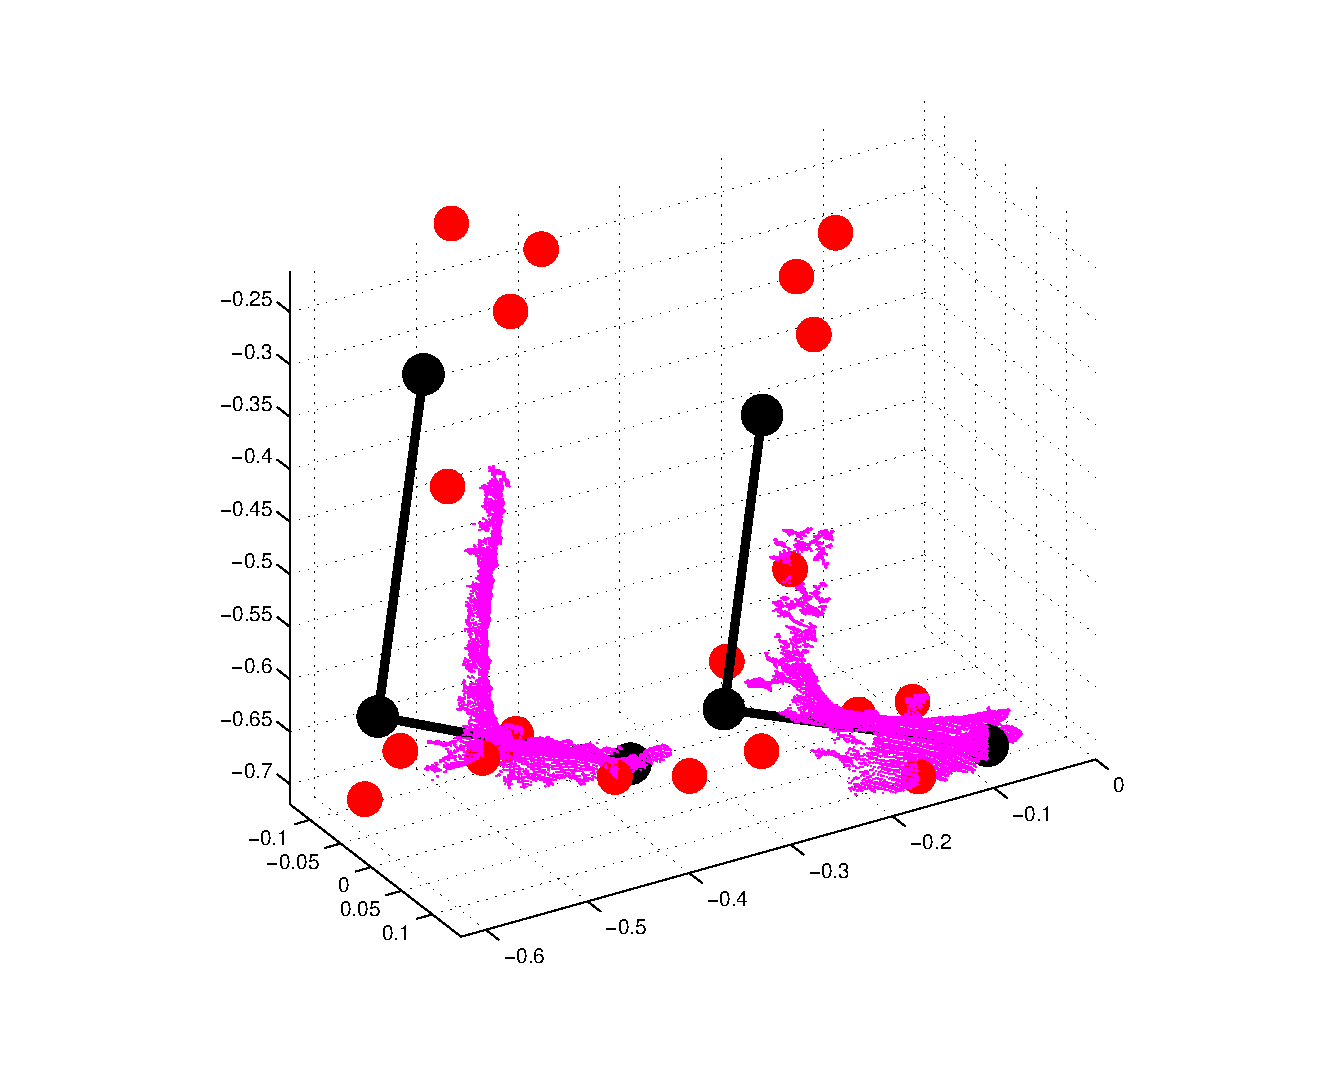
\includegraphics[width=0.45\textwidth]{images/exampleBones}
	\caption{Example of result provided by the algorithm (black bones). The kinect data are plotted in yellow and the ground truth markers are in red.}
	\label{fig:exampleBones}
\end{figure}

\section{Kalman filtering}
\label{sec:Kalman}

\subsection{Motivation}

Although the algorithm presented in the previous section can segment well the Kinect points cloud frame per frame, it does without time coherence. So, we chose to add a Kalman filter by side to smooth the trajectory and reject outliers. 

\subsection{Model and evolution matrix}
The idea is to define a state with the 3 points defining the two segments. A classical constant speed model is used. For each side, we use the following state vector:
\begin{equation}
	\mathbf{X}_k = 
	\begin{bmatrix}
		\mathbf{X_1}^T_k & \mathbf{X_1}^T_k & \mathbf{X_1}^T_k & \mathbf{V_1}^T_k & \mathbf{V_2}^T_k & \mathbf{V_3}^T_k
	\end{bmatrix}^T
\end{equation}
where $\mathbf{X_1}$ (resp. $\mathbf{X_2}$) is the vector representing the 3D Euclidean coordinates of the toe (resp. heel). $\mathbf{X_3}$ stands for the 3D coordinates of the last point of the bones representation. It is defined such that it $\mathbf{X_3}-\mathbf{X_2}$ is in the direction of the cylinder and has a predetermined norm. $\mathbf{V_1}$, $\mathbf{V_2}$ and $\mathbf{V_3}$ are the associated speeds. The evolution matrix is given by:
\begin{equation}
	\mathbf{X}_{k} =
	\begin{bmatrix}
		\mathbf{I_{9\times 9}} & \mathbf{I_{9\times 9}}\Delta t  \\
		\mathbf{0_{9\times 9}} & \mathbf{I_{9\times 9}}
	\end{bmatrix}\cdot \mathbf{X}_{k-1}
\end{equation}

\subsection{Measurement equations}
Measurement are provided by the segmentation algorithm. 3 kind of measurement can be distinguished:
\begin{enumerate}
	\item Direct measurement from the segmentation algorithm
	\item Constraint between $\mathbf{X_1}$ and $\mathbf{X_2}$: the norm of the difference is constant but unknown
	\item Constraint between $\mathbf{X_2}$ and $\mathbf{X_3}$: the norm of the difference is constant and known
\end{enumerate}

\subsubsection{Direct measurements}~\\
Direct measurements are provided by the segmentation algorithm which provides $\mathbf{X_1}$, $\mathbf{X_2}$ and $\mathbf{X_3}$. The observation matrix is obvious and is made by identity blocks for the positions and zero blocks for the speeds.

\subsubsection{Constraint between $\mathbf{X_1}$ and $\mathbf{X_2}$}~\\
In this work, we assume that the feet are like a rigid body, so that the norm of $\mathbf{X_2}-\mathbf{X_1}$ is constant. Thus, we have:
\begin{equation}
	\frac{d}{dt}\left(\left(\mathbf{X_2}-\mathbf{X_1}\right)^T\cdot\left(\mathbf{X_2}-\mathbf{X_1}\right)\right)=0
\end{equation}
So, we have the following constraint equation:
\begin{equation}
	\left(\mathbf{V_2}-\mathbf{V_1}\right)^T\cdot\left(\mathbf{X_2}-\mathbf{X_1}\right)=0
	\label{eq:constr1}
\end{equation}
Since this constraint is almost always verified, a covariance matrix close to zero is associated. This equation is non linear and the observation matrix implies to compute the Jacobian of \eqref{eq:constr1}

\subsubsection{Constraint between $\mathbf{X_2}$ and $\mathbf{X_3}$}~\\
By construction, the norm of $\mathbf{X_3} -\mathbf{X_2}$ is constant and known. So, we have the following constraint:
\begin{equation}
	\left(\mathbf{X_3}-\mathbf{X_2}\right)^T\cdot\left(\mathbf{X_3}-\mathbf{X_2}\right) = d^2
	\label{eq:constr2}
\end{equation}
where $d$ is known and fixed by advance. Similarly to the previous constraint, a covariance matrix close to zero is associated to \eqref{eq:constr2}.

\subsection{Outlier rejection}
Finally, the Kalman  prediction can be applied to outlier rejection. The idea is to compare Mahlanobis distance between the prediction of $\mathbf{X_i}_k$ and its measurement provided by the segmentation algorithm, with is the sum of the covariance matrices of the prediction and the measurement. So, we compute the following value for each point $i\in[1\dots 3]$:
\begin{equation}
	\tiny
	\left(
		\mathbf{X_i}_k^{pred} - \mathbf{X_i}_k^{meas}
	\right)^T\cdot
	\left(
		\mathbf{P_i}_k^{pred} + \mathbf{R_i}^{meas}
	\right)^{-1}\cdot
	\left(
		\mathbf{X_i}_k^{pred} - \mathbf{X_i}_k^{meas}
	\right)
	\label{eq:mahal}
\end{equation}
where $\mathbf{P_i}_k^{pred}$ is the covariance associated to the prediction of $\mathbf{X_i}_k$ (i.e. $\mathbf{X_i}_k^{pred}$) and $\mathbf{R_i}^{meas}$ is the covariance matrix associated to the measurement of $\mathbf{X_i}_k$ (i.e. $\mathbf{X_i}_k^{meas}$). The value computed in~\ref{eq:mahal} is computed to a threshold computed thanks to $\chi^2$ distribution. The measurement is rejected if the value is above the threshold. 
 
This algorithm allows us to detect and reject spurious values computed by the segmentation algorithm. For example, if the fitting strongly fails and converge to a time-inconsistent value, the Kalman filtering with outlier rejection is able to reject it.
\section{Results}

\subsection{Presentation of the experiment}
Our rollator with Kinect was tested with a person walking during two cycles of walk. A ground truth is provided by the motion capture sensor. We propose in this experiment to compute the evolution of several parameters during the walk:
\begin{itemize}
	\item The feet angles in the Kinect frame
	\item The angle between the two segments computed, that we approximate to the ankle angle
	\item The height of the heel
\end{itemize}
These parameters provide very useful information about the walk. For example, it is possible to know if the cycle is standard or not. By combining these information with the odometry, it is possible to make statistics about the length of the steps (out of the scope of this paper).

Unfortunatelly, the data collected do not correspond to a full legnth cycle walk. This is due to problem of visibility of the whole leg in the Kinect frame: our Kinect was a bit to close of the member and there was a problem of angle of view. The first problem will be corrected in the future by using a Prime sense\footnote{An other constructor of Kinect-like sensor who sells a small-range certified version of the sensor.} adapted for close measurements. The second problem will be corrected by slightly modifying the viewing angle of the sensor. To these reasons, the following results can only be considered as \textbf{preliminary results}. 

\subsection{Results analysis}
Fig.~\ref{} show the results of error in orientation of the feet. It can be seen that the elevation angle (computed with respect to the ground) is pretty well estimated (less than 5deg of error in most cases). This is an important result that show that the system may be able to pretty well estimate if a foot is on the ground or not. 

Concerning the bearing angles, the results are less precise. However, the results are globally consistent and can be used to detect anomalies in the angle feet (see fig.~\ref{}).

The ankle angle estimation is also consistent (fig.~\ref{}) even if it is a bit less precise than the feet elevation angles. 

Finally, we wanted to compare the $z$ coordinate of the heel to the $z$ coordinate of the heel computed by our model. However, we know that these two points are not exactly and that the point associated to the heel in our model is higher. To test the consistency of our model, we test if the real heel is in the axis defined by our model (fig~\ref{ }). Then, the distance between the two points should be constant.

%Finally, the $z$ trajectory computed for the toe seems coherent:\footnote{Unfortunately, there is no ground truth for this point} we can see that it is sometimes on the ground and then at a higher altitude. 

\begin{figure}
	\centering
	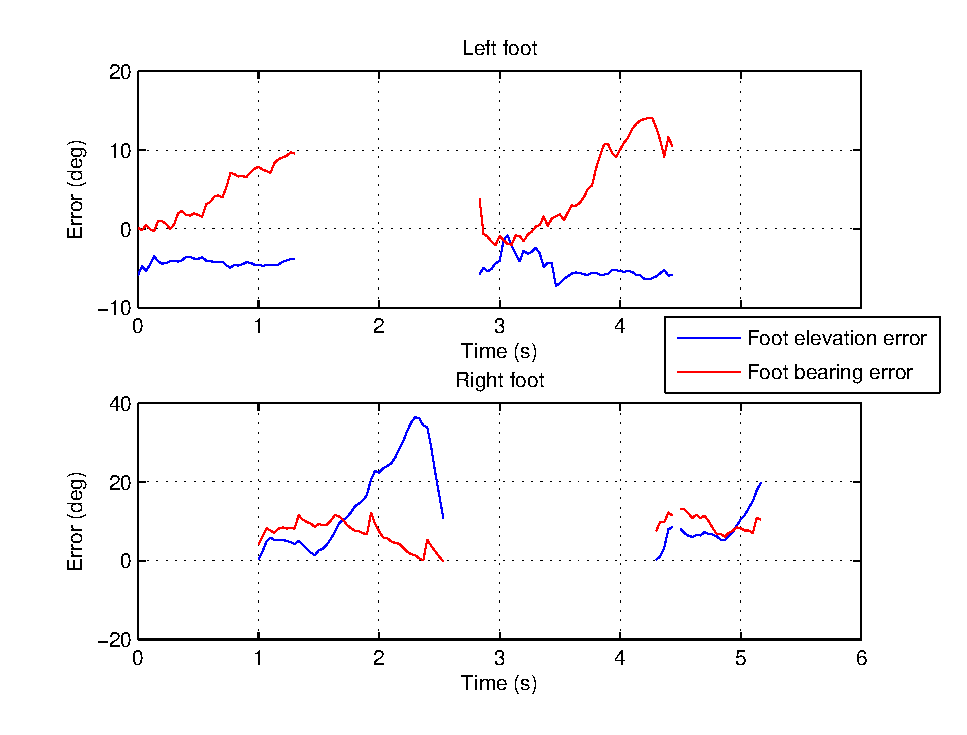
\includegraphics[width=0.45\textwidth]{images/footError}
	\caption{Orientation errors for the feet}
	\label{fig:footError}
\end{figure}

\begin{figure}
	\centering
	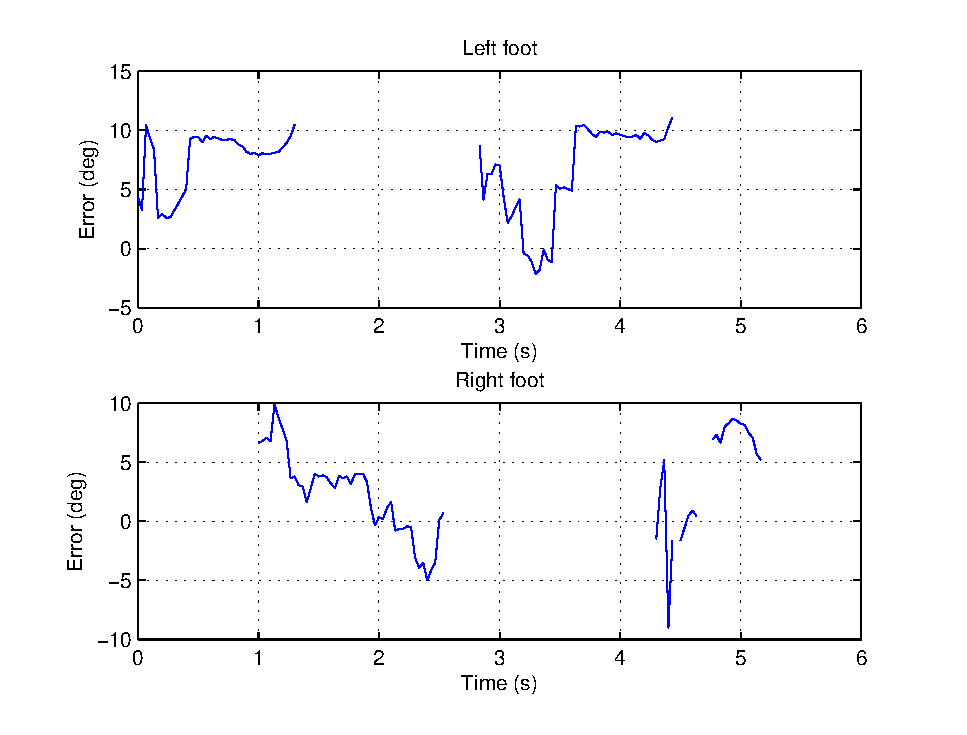
\includegraphics[width=0.45\textwidth]{images/errorAnkle}
	\caption{Error on ankle angle estimation}
	\label{fig:errorAnkle}
\end{figure}

\begin{figure}
	\centering
	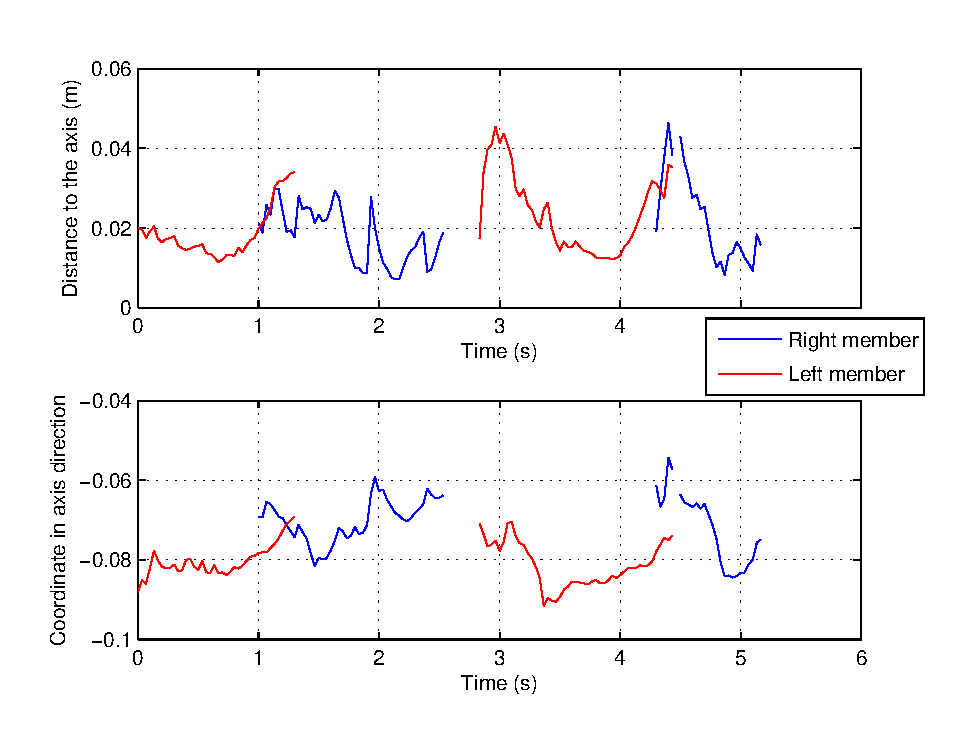
\includegraphics[width=0.45\textwidth]{images/heelError}
	\caption{Difference between real heel position and estimation}
	\label{fig:heelError}
\end{figure}

\begin{figure}
	\centering
	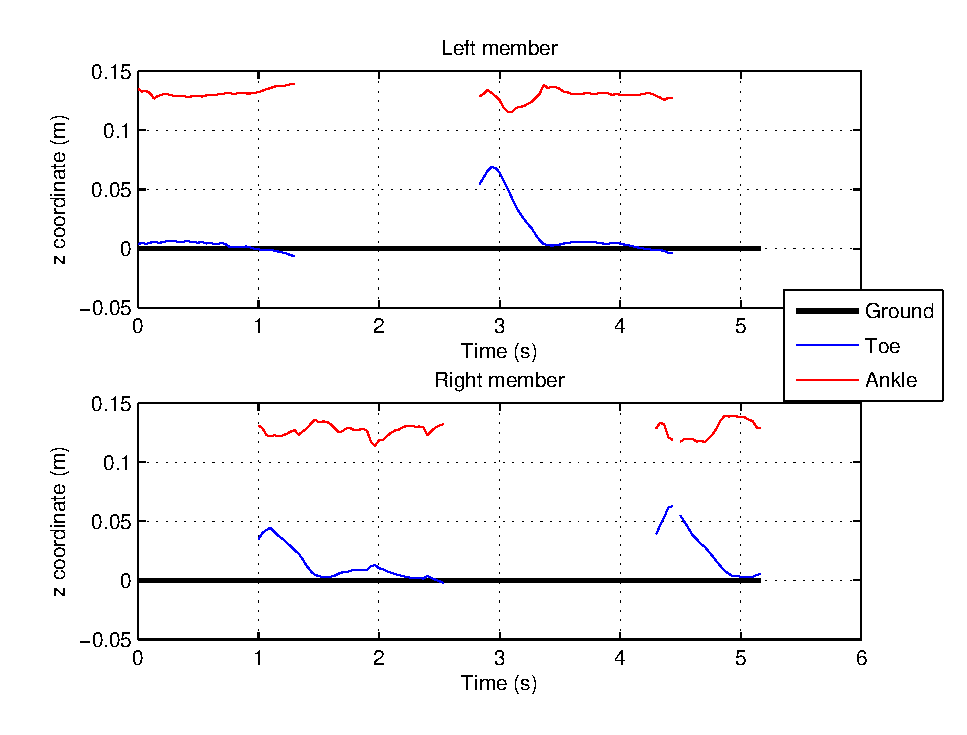
\includegraphics[width=0.45\textwidth]{images/exProfile2}
	\caption{$z$ trajectory of the toes and ``heels'' estimated by the algorithm}
	\label{fig:exProfile}
\end{figure}
\section{Conclusion}

\bibliographystyle{IEEEtran} 
\bibliography{biblio.bib}

% LIRMM D. Guiraud, P. Poignet, C. Azevedo Stimultation électrique fonctionnelle, étude de la posture
% P.B Wieber INRIA Grenoble

\end{document}

